\documentclass{amsart}[12pt]
\usepackage{amsmath, amsfonts, tikz, natbib, array}
\oddsidemargin=0in \evensidemargin=0in
\textwidth=6.6in \textheight=8.7in

\title{A variation on the Chamberlin Trimetric map projection}
\author{B R S Recht}
\date{October 2019}

\begin{document}

\begin{abstract}
   A variation of the Chamberlin Trimetric map projection is presented. This
   projection amounts to a linear transformation of the distances from a point
   to three control points, and is simpler and more stable than the Chamberlin
   projection. It also allows for an inverse projection in the spherical
   approximation that only requires numerical estimation of one parameter.
\end{abstract}
\maketitle

\section{Introduction}

\cite{christensen}\cite{snyder87}\cite{snyder89}

\section{Derivation of forward projection}
This derivation will make heavy use of basic linear algebra: refer to a basic
text on linear algebra, such as \cite{strang}, if anything is
unfamiliar.

Let $\mathbf v$ be a point on some geodetic datum, and let $\mathbf p = [x, y]$
be a point in the Euclidean plane. Let $d(\mathbf v_a, \mathbf v_b)$ be the
geodesic distance between the points $\mathbf v_a$ and $\mathbf v_b$ on that
datum. Let $\|\mathbf p\| = \sqrt{x^2 + y^2}$ be the Euclidean norm of the point
$\mathbf p$, such that $\|\mathbf p_a - \mathbf p_b\|$
is the Euclidean distance between the points $\mathbf p_a$ and $\mathbf p_b$.

Let $\mathbf v_1$, $\mathbf v_2$, $\mathbf v_3$ be control points on the sphere,
and $\mathbf p_1 = [x_1, y_1]$ etc. be the image of those control points on the
plane, such that $d(\mathbf v_i, \mathbf v_j) = \|\mathbf p_i - \mathbf p_j\|$
for all $i$ and $j$ in ${1, 2, 3}$. The triangles with vertices at $\mathbf v_i$
or $\mathbf p_i$ will be called the control triangles (spherical or planar
control triangle, respectively, if the distinction is important). Without loss
of generality, also assume that $\|\mathbf p_i\|$ is the same for all $i$, such
that the center of the circumcircle of the control triangle lies at the origin.
(This just removes a translation in the plane in order to simplify the formula;
false northing and easting can be added later.)

Let $r_i = d(\mathbf v_i, \mathbf v)$ be the geodesic distance from
$\mathbf v_i$ to $\mathbf v$, but also the radius of a circle that is centered
at $\mathbf v_i$ and $\mathbf v$ lies on its boundary. The original Chamberlin
projection draws a circle of radius $r_i$ around each point $\mathbf p_i$,
forming a small triangle with circular arcs for edges, and chooses a point
$\mathbf p$ within that small triangle. Originally, in the 1950s when manual
plotters were used, the exact definition of this point was not important, but Christensen
\cite{christensen} and most modern implementations (e.g. Proj \cite{proj}) use
the centroid of the triangle formed by the points where each pair of circles
intersect. Of course, each pair of circles intersects in (at most) two places,
so the implementation must take care to choose the point of intersection that
lies on the small triangle and not the other one.

\begin{figure}%[!htbp]
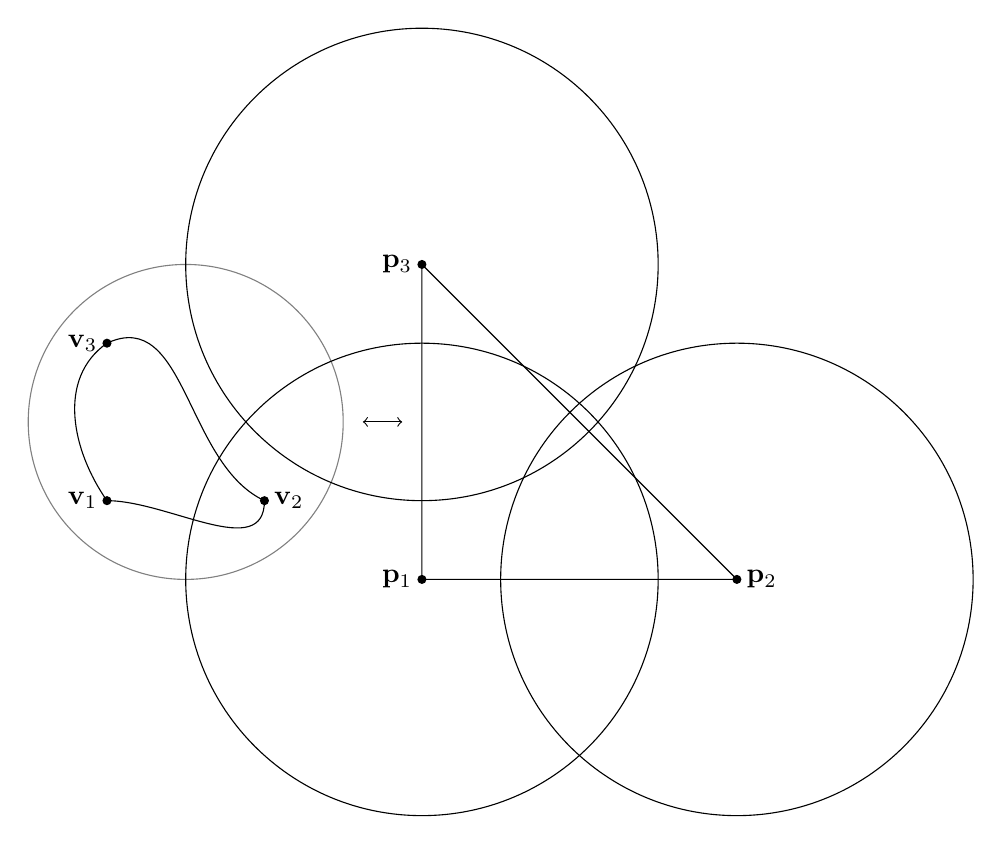
\begin{tikzpicture}
  \draw [gray] (2,2) circle [radius=2];
  \draw (1, 1) to [out=0, in=-90]
  (3, 1) to [out=155, in=25]
  (1, 3) to [out=215, in=125]
  (1, 1);
  \draw[fill] (1,1) circle [radius=0.05] node[anchor=east] {$\mathbf v_1$};
  \draw[fill] (3,1) circle [radius=0.05] node[anchor=west] {$\mathbf v_2$};
  \draw[fill] (1,3) circle [radius=0.05] node[anchor=east] {$\mathbf v_3$};

  \draw [<->] (4.25,2) -- (4.75,2);
  \draw (5, 0) -- (9, 0) -- (5, 4) -- (5, 0);
  \draw[fill] (5,0) circle [radius=0.05] node[anchor=east] {$\mathbf p_1$};
  \draw[fill] (9,0) circle [radius=0.05] node[anchor=west] {$\mathbf p_2$};
  \draw[fill] (5,4) circle [radius=0.05] node[anchor=east] {$\mathbf p_3$};
  \draw (5,0) circle [radius=3];
  \draw (9,0) circle [radius=3];
  \draw (5,4) circle [radius=3];

\end{tikzpicture}
\caption{Depiction of Chamberlin projection.}
\label{fig:chamberlin}
\end{figure}

One can make two observations on this configuration of circles in the plane. One
is that the two points of intersection of each pair of circles are symmetric
about the triangle edge between the two control points. The other is that, if
one draws a line through the two points of intersection of each pair of circles,
that line is perpendicular to the triangle edge, and once the lines are drawn
for each pair of circles, the three lines appear to meet at the same point.
(That observation will be proven true momentarily.) Although that point is not
necessarily within the small triangle, it is for most points within the control
triangle.

Suppose that $\mathbf p_1 = [-1,0]$ and $\mathbf p_2 = [1,0]$. Then the points
of intersection of the circles with radius $r_1$ and $r_2$ are given as so:
\begin{equation}\begin{split}
x =& \frac{r^2_1 - r^2_2}{4}\\
y =& \pm \frac{1}{4} \sqrt{-
\left(r_1 - r_2 - 2\right)
\left(r_1 - r_2 + 2\right)
\left(r_1 + r_2 - 2\right)
\left(r_1 + r_2 + 2\right)}
\end{split}\end{equation}
Note that there is not necessarily a real solution for $y$. In that case, the
circles do not intersect.

If a line passing through the two points of intersection is drawn, it intersects
the triangle edge from $\mathbf p_1$ to $\mathbf p_2$ perpendicularly at
the point with $x$ as above and $y=0$: call that point $\mathbf p_{12}$. In
general form, one can use linear interpolation to determine the point of
perpendicular intersection $\mathbf p_{ij}$ as so:
\begin{equation}\label{eq:pij}
\mathbf p_{ij} = \mathbf p_i \frac{1-t_{ij}}{2} + \mathbf p_j \frac{1+t_{ij}}{2}
\end{equation}
\begin{equation}
t_{ij} = \frac{r_i^2 - r_j^2}{\| \mathbf p_i - \mathbf p_j \|^2}
\end{equation}
Note that this is defined for all $r_i$, regardless of whether the circles
intersect.

The lines passing through $\mathbf p_{ij}$ and parallel to the line from
$p_i$ to $p_j$ all meet at the same point. This can be proven with a simple
triangle theorem sometimes attributed to Carnot: such lines meet at a single
point if and only if \cite{posamentier}\cite{wohlgemuth}
\begin{equation}
  \|\mathbf p_1 - \mathbf p_{12}\| +
  \|\mathbf p_2 - \mathbf p_{23}\| +
  \|\mathbf p_3 - \mathbf p_{31}\| =
  \|\mathbf p_2 - \mathbf p_{12}\| +
  \|\mathbf p_3 - \mathbf p_{23}\| +
  \|\mathbf p_1 - \mathbf p_{31}\|
\end{equation}
for points $\mathbf p_{ij}$ lying on the edge between $\mathbf p_i$ and
$\mathbf p_j$. Plugging in Equation \ref{eq:pij} and simplifying proves that
these lines satisfy this theorem.

The equation of the line passing from $\mathbf p_i$ to $\mathbf p_j$ is:
\begin{equation}
y (x_i - x_j) - x (y_i - y_j) - x_i y_j - x_j y_i = 0.
\end{equation}
Thus, the equation of the line perpendicular to that line and passing through
the point $\mathbf p_{ij}$ can be found to be
\begin{equation}
y (y_i - y_j) + x (x_i - x_j) + \frac{r_i^2 - r_j^2}{2} = 0.
\end{equation}
Combining the equation of each perpendicular line creates a linear system.
It is an overdetermined system of 3 equations in 2 variables, but since all 3
perpendicular lines meet at the same point as proven above, it has a solution.
Ultimately this system can be solved for $\mathbf p$ to define a map projection
as follows. Let $\mathbf P$ be a 3x2 matrix having $\mathbf p_i$ as its $i$th
column. Then:
\begin{equation}\label{eq:forward}
\mathbf p = \mathbf M \begin{bmatrix} r^2_1 & r^2_2 & r^2_3 \end{bmatrix}^\top,
\end{equation}
\begin{equation}
\mathbf M = \frac{1}{2T}
\begin{bmatrix} y_3 - y_2 & y_1 - y_3 & y_2 - y_1 \\
x_2 - x_3 & x_3 - x_1 & x_1 - x_2 \end{bmatrix} = \frac{1}{2T}
\begin{bmatrix} 0 & -1  \\
1 & 0 \end{bmatrix}
\mathbf P
\begin{bmatrix} 0 & -1 & 1 \\
1 & 0 & -1 \\
-1 & 1 & 0 \end{bmatrix},
\end{equation}
\begin{equation}
T = \begin{vmatrix} x_1 & x_2 & x_3 \\
 y_1 & y_2 & y_3 \\
 1 & 1 & 1
\end{vmatrix}.
\end{equation}
$T$ is equal to twice the area of the Euclidean control triangle. $T$ is zero
if all the control points lie on a line, and is very small if the control
points are very close to each other, in which case the matrix $\mathbf M$ is
undefined or numerically unstable.
(Of course, those are not typical use cases for the Chamberlin projection.)

The matrix $\mathbf M$ has a (right) nullspace spanned by the vector $[1,1,1]$.
In general, this implies this projection is not one-to-one for all possible
values of $r_i$: in particular, if $r_1 = r_2 = r_3$, then $\mathbf p = [0,0]$.
Of course, not all values of $r_i$ correspond to actual points on the datum,
but this projection will be observed later on to have overlap for some points
outside the control triangle, much like the Chamberlin projection.
(Again, the Chamberlin projection is not commonly used to project the entire
earth, except for demonstration purposes.)

\section{Inverse}
Given $\mathbf p$, we start to invert the projection as so:
\begin{equation}\label{eq:inverse}
\begin{bmatrix} k_1 & k_2 & k_3

\end{bmatrix}^\top = \mathbf M^+ \mathbf p,
\end{equation}
\begin{equation}
\mathbf M^+ = \frac{2}{3}
\begin{bmatrix} 2x_1 - x_2 - x_3 & 2y_1 - y_2 - y_3 \\
-x_1 + 2x_2 - x_3 & -y_1 + 2y_2 - y_3 \\
-x_1 - x_2 + 2x_3 & -y_1 - y_2 + 2y_3
\end{bmatrix} = \frac{2}{3}
\begin{bmatrix} -2 & 1 & 1 \\
1 & -2 & 1 \\
1 & 1 & -2
\end{bmatrix}
\mathbf P^\top
\end{equation}
$k_i = r^2_i - h$ for some value $h$. This is a general solution to inverting
Equation \ref{eq:forward}, thus the free parameter $h$. $\mathbf M^+$ is the
pseudoinverse of $\mathbf M$ and vice versa. Because $\mathbf M^+$ has a left
nullspace spanned by the vector $[1,1,1]$, it follows that $\sum_i k_i = 0$,
which can be used to calculate $k_i$ more efficiently.

By plugging Equation \ref{eq:forward} into Equation \ref{eq:inverse}, we can
find that $h = \frac{1}{3}\sum_i r^2_i$. Unfortunately, if one attempts to
solve for $r_i$ given $k_i$, they find another general solution with one free
parameter, putting them right back where they started. It turns out that
information about the geoid needs to be introduced to determine $r_i$ and
$\mathbf v$. In the following, this is done with spherical approximation, and
the case of an ellipsoid is discussed.

\subsection{With spherical approximation}
If treating the earth as a unit sphere, then let $\mathbf v = [x, y, z]$ be a
Euclidean vector such that its norm is 1:
$\|\mathbf v \|= \sqrt{x^2 + y^2 + z^2} = 1$.
In that case, spherical geometry allows an analytic way to determine a vector
$\mathbf v$ given $r_i$. For this section, let $r_i$ have units of radians of
arc on the surface of the sphere. The circle of points $\mathbf v$ at distance
$r_0$ from a point $\mathbf v_0$ is simply the circle where a plane intersects
the sphere. This plane may be specified as so:
\begin{equation}
  \mathbf v_0 \cdot \mathbf v = \cos\left(r_0\right).
\end{equation}
Clearly, replacing $\mathbf v_0$ with $\mathbf v_i$ and $r_0$ with $r_i$ for
each $i$ gives a linear system. Let $\mathbf V$ be the matrix having
$\mathbf v_i$ as its $i$th column. Thus,
\begin{equation}
  \mathbf v = \mathbf V^{-1} \begin{bmatrix} \cos\left(r_1\right) \\
  \cos\left(r_2\right) \\
  \cos\left(r_3\right)
  \end{bmatrix}
\end{equation}
$\mathbf V^{-1}$ is undefined or numerically ill-behaved if the control points
lie on a line or are very close together. It is also undefined if the points all
lie on a great circle of the sphere: in that case, there are two points that
satisfy the values of $r_i$. Again, those are not typical use cases for
the Chamberlin projection.

For the point to lie on the unit sphere, $\|\mathbf v\| = 1$. Let $\mathbf c$
be a vector with $i$th component $\cos\left(r_i \right)$. Then,
\begin{equation}
  \mathbf c^\top \left(\mathbf V^\top \mathbf V\right )^{-1} \mathbf c = 1
\end{equation}
Make the substitution $r_i = \sqrt{k_i + h}$. The result is a little opaque,
but we now have an equation with one unknown, $h$. Some obvious bounds can be
placed on $h$. In units of radians, $0 \le r_i \le \pi$. Since this must hold
for every $r_i$, it follows that
$$
h_{\min} = -\min_i k_i \le h \le \pi^2 - \max_i k_i = h_{\max}
$$.
Within these bounds, there may be at most two solutions for $h$. In most
applications, the solution with smaller $h$, nearer to the control triangle, is
the desirable one. Let
$\mathbf A = \left(\mathbf V^\top \mathbf V\right )^{-1}$,
where $\mathbf A$ is symmetric and positive semi-definite, and
$f(h) = \mathbf c^\top \mathbf A \mathbf c - 1$. The derivative of $f(h)$ is
\begin{equation}
  f'(h) = -\mathbf c^\top \mathbf A \mathbf b
\end{equation}
where $\mathbf b$ is the vector with $i$th component
$\mathrm{sinc}\left(\sqrt{k_i + h}\right)$, and the function $\mathrm{sinc} (x)$
is defined as so:
\begin{equation}
\mathrm{sinc} (x) = \begin{cases}
      1 & \text{if}\ x=0, \\
      \frac{\sin x}{x} & \text{otherwise}.
    \end{cases}
\end{equation}
Note that $f'(h)$ and $f(h)$ share many of the same terms, making the
calculation more efficient. If needed for numerical purposes, the compositions
of trig functions with square root can be smoothly extended to negative values:
when $x<0$, $\cos \sqrt{x} = \cosh \sqrt{-x}$
and $\frac{\sin \sqrt{x}}{\sqrt{x}} = \frac{\sinh \sqrt{-x}}{\sqrt{-x}}$.

Given all the preceding, Newton's method can be applied to solve for $h$.
Using $h_{\min}$ as an initial guess, a good approximation is achieved for
points inside the control triangle within only a few iterations. Better initial
guesses are possible, but don't appear to be worth the cost of calculation.
Convergence is somewhat slower further away from the control triangle, and is
worst at the boundary of the projection. This is expected: at the boundary, the
function reaches a minimum at the same place as its root, $f(h)=f'(h)=0$, and
Newton's method converges at a merely linear rate.\cite{burden}

 (insert graphs of f(h) here)

\subsection{Without spherical approximation}
The method for spheres is not extensible to ellipsoidal datums. Geodesic
circles cannot in general be described as the intersection of a plane and a
surface. Also, we can no longer make the assumption that the Euclidean norm
$\|\mathbf v\|$ is constant. In general, these sort of problems are harder
on an ellipsoid than a sphere: calculating geodesic distances, for example,
typically involves elliptic functions or iterative approximations to such
functions. Geodesic circles are usually calculated in most software by
extending a number of lines from a center point and using the endpoints as an
approximation of the circle. It is not surprising that an analytic form, or
form with an easy numerical iteration, is not available here.

The spherical approximation is reasonably close to an ellipsoidal
calculation. (insert round-trip analysis here)

\section{Comparison}

\section{Conclusion}

spherical inversion is no worse than that in Snyder equal area \cite{snyder92}

\bibliographystyle{plain}
\bibliography{references}

\end{document}
